%%====================================================================
%% Solving 2048: Classical RL vs. LLM-Guided RLVR
%% AAAI-26 Format
%%====================================================================
\documentclass[letterpaper]{article}
\usepackage{aaai26}
\usepackage{amsmath,amssymb,amsfonts}
\usepackage{graphicx}
\usepackage{xcolor}
\usepackage{booktabs}
\usepackage{algorithm}
\usepackage{algpseudocode}
\usepackage{subcaption}
\usepackage{hyperref}
\usepackage{cite}
\usepackage{multirow}
\usepackage{array}
\usepackage{colortbl}
\usepackage{textcomp}

\definecolor{dqncolor}{HTML}{D35400}
\definecolor{rlvrcolor}{HTML}{7D3C98}

\begin{document}

\title{Solving 2048: A Comparative Study of\\Classical Reinforcement Learning and LLM-Guided RLVR}

\author{
Shriman Raghav \quad Gautham Ramkumar \\
MS Robotics, Khoury College of Computer Sciences \\
Northeastern University, Boston, MA \\
\texttt{srinivasan.shrim@northeastern.edu}
}

\maketitle

%%====================================================================
\begin{abstract}
We present a systematic comparison of classical reinforcement learning and Reinforcement Learning with Verifiable Rewards (RLVR) on the 2048 puzzle game. Six classical agents -- Deep Q-Network (DQN), Proximal Policy Optimization (PPO), Advantage Actor-Critic (A2C), Quantile Regression DQN (QR-DQN), discrete Soft Actor-Critic (SAC), and Semi-gradient SARSA with linear function approximation -- are benchmarked against Qwen2.5 language models (0.5B and 1.5B parameters) fine-tuned via Group Relative Policy Optimization (GRPO). All deep classical agents share an identical three-layer CNN backbone (330K parameters) to isolate algorithmic effects. We evaluate at three levels: 1M training steps, 5M training steps, and unlimited-attempt hunt mode. DQN achieves the highest classical score (avg 7,744 at 5M steps; tile 2048 in hunt mode), while Semi-gradient SARSA with only 120 parameters outperforms all deep on-policy methods, validating Sutton \& Barto's thesis that engineered features trump raw network capacity when data is scarce. GRPO-trained LLMs demonstrate a clear model-scale dependence ($3\times$ parameters $\to$ $3.3\times$ score), but classical agents remain $\sim$400$\times$ faster at inference. We release a live dashboard and complete codebase for reproducibility.
\end{abstract}

%%====================================================================
\section{Introduction}
\label{sec:intro}

The tile-sliding puzzle 2048 was introduced in 2014 by Gabriele Cirulli and quickly attracted attention from the AI community. On every turn the player selects one of four cardinal directions; all tiles slide accordingly, identical adjacent tiles merge (doubling their value), and a fresh 2 or 4 tile spawns at a uniformly random empty cell. The game terminates when no legal move remains.

Despite its compact $4{\times}4$ board, 2048 poses fundamental challenges for learning agents. The state space is vast (${\sim}10^{19}$ configurations), rewards are sparse and delayed (hundreds of preparatory moves may earn nothing before a single high-value merge), and stochastic tile spawns make planning difficult. These properties make 2048 an ideal benchmark for comparing fundamentally different learning paradigms.

Recently, a new paradigm has emerged: Reinforcement Learning with Verifiable Rewards (RLVR). Instead of training a neural network policy via environment interaction, RLVR fine-tunes large language models (LLMs) to generate chain-of-thought reasoning validated by deterministic reward functions~\cite{guo2025deepseek, wen2025rlvr}. While RLVR has yielded breakthroughs in mathematical reasoning, its application to spatial strategy games remains largely unexplored.

This paper asks three questions: \textbf{(Q1)}~How do six classical RL algorithms compare on 2048 when architectural confounds are removed? \textbf{(Q2)}~Can small LLMs (0.5B--1.5B parameters) acquire 2048 strategy through GRPO alone, without using proprietary LLM APIs? \textbf{(Q3)}~What are the fundamental trade-offs between classical RL's throughput and RLVR's interpretability?

Our contributions include:
\begin{enumerate}
    \item A controlled benchmark of six classical agents and two GRPO-LLM agents on a unified 2048 environment with clear 1M/5M/hunt-mode evaluation tiers.
    \item Demonstration that Semi-gradient SARSA (Sutton \& Barto, Algorithm~10.1~\cite{sutton2018rl}) with 120 parameters outperforms all deep on-policy methods with 330K+ parameters.
    \item A GRPO training pipeline for locally deployed LLMs with analysis of model-scale dependence and spatial reasoning failures.
    \item Evidence that on-policy methods (PPO, A2C) actively degrade with extended training on 2048, losing 9--12\% score from 1M to 5M steps.
    \item A live web dashboard for step-by-step replay visualization.
\end{enumerate}

%%====================================================================
\section{Background}
\label{sec:background}

\subsection{Markov Decision Process Formulation}

The 2048 game is modeled as a finite-horizon MDP $(\mathcal{S}, \mathcal{A}, P, R, \gamma)$ where:
\begin{itemize}
    \item $\mathcal{S}$: Board states, encoded as 16-channel binary tensors $\mathbf{x}\in\{0,1\}^{16\times4\times4}$ for CNN agents, or ASCII text for LLM agents.
    \item $\mathcal{A} = \{\text{UP}, \text{RIGHT}, \text{DOWN}, \text{LEFT}\}$: Four discrete actions.
    \item $P(s'|s,a)$: Deterministic tile-sliding with stochastic spawn (90\% tile-2, 10\% tile-4 at random empty cell).
    \item $R(s,a,s')$: Score-delta plus milestone bonuses (+50 at 256, +100 at 512, +200 at 1024) and $-1$ penalty for invalid moves.
    \item $\gamma = 0.99$: Discount factor.
\end{itemize}

\subsection{Value-Based Methods}

Value-based approaches estimate the action-value function $Q^\pi(s,a) = \mathbb{E}_\pi[\sum_{t=0}^\infty \gamma^t r_t | s_0=s, a_0=a]$ and act greedily. DQN~\cite{mnih2015human} parameterizes $Q$ as a neural network and stabilizes learning via experience replay and a frozen target network. QR-DQN~\cite{dabney2018distributional} extends DQN by modeling the full return distribution via quantile regression.

\subsection{Policy-Gradient Methods}

Policy-gradient methods directly optimize the policy $\pi_\theta(a|s)$. PPO~\cite{schulman2017proximal} uses a clipped surrogate objective with Generalized Advantage Estimation (GAE). A2C~\cite{mnih2016asynchronous} is a synchronous actor-critic using $n$-step returns. SAC~\cite{haarnoja2018soft} augments the RL objective with an entropy bonus, encouraging exploration.

\subsection{Linear Function Approximation}

Sutton \& Barto~(\S9.3,~\cite{sutton2018rl}) describe linear function approximation where $\hat{q}(s,a,\mathbf{w}) = \mathbf{w}_a^\top\phi(s)$, with $\phi(s)$ a hand-crafted feature vector. Semi-gradient SARSA (Algorithm~10.1) updates weights using only the gradient of the prediction, not the bootstrap target. Under linear FA, semi-gradient SARSA converges to a TD fixed point with bounded approximation error~(\S9.4).

\subsection{RLVR and Group Relative Policy Optimization}

RLVR trains LLMs using rewards from deterministic verifiers rather than human feedback~\cite{guo2025deepseek}. Group Relative Policy Optimization (GRPO)~\cite{shao2024deepseekmath} eliminates the critic network by normalizing advantages within a group of $G$ sampled completions per prompt:
\begin{equation}
    \hat{A}_i = \frac{r_i - \mu_G}{\sigma_G + \epsilon}
    \label{eq:grpo_adv}
\end{equation}
This replaces the critic's state-dependent baseline with a sample-based, prompt-specific baseline.

%%====================================================================
\section{Related Work}
\label{sec:related}

\textbf{Classical approaches to 2048.}
Szubert \& Ja\'skowski~\cite{szubert2014temporal} use temporal-difference learning with n-tuple networks, achieving strong performance via tabular value approximation over board patterns. Saligram et al.~\cite{saligram2025delayed} apply DQN with delayed-reward shaping. Our work differs by comparing six algorithms on a shared backbone, isolating the learning algorithm from architectural choices.

\textbf{Deep RL for games.}
Mnih et al.~\cite{mnih2015human} demonstrated human-level Atari play with DQN. Subsequent work introduced distributional RL~\cite{dabney2018distributional}, entropy-regularized policies~\cite{haarnoja2018soft}, and trust-region methods~\cite{schulman2017proximal}. We evaluate all four paradigms on a single game with matched architectures.

\textbf{LLMs for game-playing.}
Hu et al.~\cite{hu2025lmgame} benchmark LLMs on diverse games including 2048, finding that even large models struggle with spatial reasoning. Our work extends this by \emph{training} LLMs via GRPO rather than prompting pretrained models, and directly comparing the trained LLM against classical RL agents under controlled conditions.

\textbf{RLVR.}
DeepSeek-R1~\cite{guo2025deepseek} showed that GRPO can incentivize reasoning in LLMs using verifiable rewards. DeepSeekMath~\cite{shao2024deepseekmath} applied GRPO to mathematical reasoning. We extend RLVR to spatial strategy games and quantify the gap between RLVR and classical approaches.

%%====================================================================
\section{Project Description}
\label{sec:method}

\subsection{Environment}

We implement a custom 2048 Gymnasium~\cite{towers2024gymnasium} environment. For CNN agents, the board is encoded as a 16-channel binary tensor (Eq.~\ref{eq:obs}):
\begin{equation}
    x_{k,i,j} = \mathbb{1}[B_{i,j} = 2^k], \quad k=0,\ldots,15
    \label{eq:obs}
\end{equation}
For LLM agents, the board is serialized as a labeled ASCII grid with current score and max tile.

\subsection{Shared CNN Backbone}

Every deep classical agent uses the same three-layer convolutional feature extractor: Conv2D($16 \to 128$, $2{\times}2$) $\to$ ReLU $\to$ Conv2D($128 \to 128$, $2{\times}2$) $\to$ ReLU $\to$ Conv2D($128 \to 128$, $2{\times}2$) $\to$ ReLU $\to$ FC($128 \to 256$). This produces a 256-dimensional feature vector; each algorithm appends its own task-specific heads. The shared backbone ensures performance differences reflect the \emph{learning algorithm}, not network capacity.

\subsection{Classical Agents}

\subsubsection{DQN (Custom PyTorch).}

Our DQN uses a custom PyTorch implementation rather than Stable-Baselines3 (SB3) because SB3's DQN lacks direct Q-value masking for invalid actions (it only supports action-space wrappers). Our implementation masks invalid Q-values to $-\infty$ \emph{inside the forward pass}, enabling proper $\varepsilon$-greedy selection over legal moves only.

Hyperparameters: replay buffer 100K, batch size 64, $\varepsilon$: $1.0 \to 0.01$ over 100K steps, target sync every 1K steps, learning rate $10^{-4}$ (Adam), gradient clipping 1.0.

\subsubsection{SAC -- Discrete (Custom PyTorch).}

Standard SAC~\cite{haarnoja2018soft} targets continuous actions. We implement the discrete adaptation of Christodoulou~\cite{christodoulou2019soft} with categorical policies, twin Q-networks, and automatic temperature tuning. This required custom code because SB3 does not natively support discrete SAC with invalid action masking in the policy distribution.

Hyperparameters: replay buffer 200K, batch size 256, Polyak $\tau=0.005$, learning rate $10^{-4}$, warmup 10K steps, target entropy $0.4 \cdot \log|\mathcal{A}|$.

\subsubsection{PPO -- MaskablePPO (Stable-Baselines3).}

We use SB3's MaskablePPO~\cite{raffin2021stable}, which natively supports action masking via environment-provided masks.

Hyperparameters: rollout 2048 steps $\times$ 8 parallel envs, batch size 64, 10 epochs per update, learning rate $3{\times}10^{-4}$, GAE $\lambda=0.95$, clip $\epsilon=0.2$, entropy coefficient $c_e=0.01$.

\subsubsection{A2C (Stable-Baselines3).}

A2C~\cite{mnih2016asynchronous} is on-policy actor-critic without PPO's clipping mechanism.

Hyperparameters: 5-step returns, learning rate $7{\times}10^{-4}$, entropy coefficient 0.01, value coefficient 0.5.

\subsubsection{QR-DQN (SB3-Contrib).}

QR-DQN~\cite{dabney2018distributional} models the return distribution via $N{=}50$ quantiles, outputting $4{\times}50{=}200$ values.

Hyperparameters: buffer 100K, batch 64, learning rate $10^{-4}$, target sync every 1K steps, $\varepsilon$: $1.0 \to 0.05$ over 10\% of training.

\subsubsection{Semi-gradient SARSA (Custom NumPy).}

Following Sutton \& Barto, Algorithm~10.1~\cite{sutton2018rl}, we implement episodic semi-gradient SARSA with linear function approximation. The agent maintains $\mathbf{w} \in \mathbb{R}^{4\times30}$ (120 parameters total) mapping a 30-dimensional feature vector $\phi(s)$ to Q-values:
\begin{equation}
    \hat{q}(s,a,\mathbf{w}) = \mathbf{w}_a^\top \phi(s)
\end{equation}

The feature vector $\phi(s)$ encodes 30 dimensions following Sutton \& Barto's guidance on feature construction~(\S9.5): 16 log-tile values, empty ratio, merge potential, 4 monotonicity scores, max-tile indicator, corner bonus, 3 tile distribution statistics, smoothness, snake-pattern score, and edge-tile sum. The semi-gradient update rule~(\S10.1) differentiates only through the prediction:
\begin{equation}
    \mathbf{w}_{a_t} \leftarrow \mathbf{w}_{a_t} + \alpha \delta_t \phi(s_t), \quad \delta_t = r_t + \gamma \hat{q}(s_{t+1}, a_{t+1}) - \hat{q}(s_t, a_t)
\end{equation}

Hyperparameters: step-size $\alpha=10^{-3}$, $\varepsilon$-decay 0.99995/step, $\varepsilon_{\min}=0.05$.

\subsection{GRPO-Trained LLM Agent}

\subsubsection{Why Local GRPO, Not an LLM API?}

We train LLMs locally via GRPO rather than using proprietary APIs (e.g., OpenAI, Anthropic) for three reasons:

\begin{enumerate}
    \item \textbf{Policy gradient access.} GRPO requires computing per-token log-probabilities $\log\pi_\theta(o_{i,t}|q, o_{i,<t})$ and their gradients to form the importance ratio $r_t^i(\theta) = \pi_\theta / \pi_{\theta_{\text{old}}}$. Commercial APIs do not expose model weights or gradient computation; only logit/log-prob outputs are sometimes available, which is insufficient for the clipped PPO-style policy update.
    \item \textbf{Cost.} GRPO generates $G{=}4$ completions per prompt across 300 training steps, totaling $\sim$1,200 forward passes per epoch. At API pricing (\$0.10--\$1.00 per 1K tokens), this training loop would cost \$100--\$500 per experiment, making iterative hyperparameter tuning infeasible on a student budget.
    \item \textbf{Reproducibility.} Local deployment with fixed random seeds and quantization settings ensures deterministic training. API-served models may change versions silently, undermining reproducibility.
\end{enumerate}

\subsubsection{Model and Training.}

We fine-tune Qwen2.5-0.5B-Instruct (494M params) and Qwen2.5-1.5B-Instruct (1.8B params)~\cite{qwen2024} using 4-bit NF4 quantization via Unsloth~\cite{unsloth2024} with LoRA adapters ($r{=}32$, $\alpha{=}32$). The GRPO loss follows Equation~\ref{eq:grpo_adv} with a KL penalty:
\begin{equation}
    \mathcal{L}_{\text{GRPO}}(\theta) = \mathbb{E}_q\!\left[\frac{1}{G}\sum_{i=1}^G \frac{1}{|o_i|}\sum_{t=1}^{|o_i|}\!\left(L_t^{\text{clip}} - \beta D_{\text{KL}}\right)\right]
\end{equation}
where $L_t^{\text{clip}} = \min(r_t^i \hat{A}_i, \text{clip}(r_t^i, 1{\pm}\epsilon)\hat{A}_i)$ and $\beta{=}0.04$.

\subsubsection{Reward Scheduling.}

The reward function uses three stages to avoid cold-start collapse: (1)~format compliance (XML tags, weight 0.5), (2)~direction validity (weight 0.5), (3)~game reward ($\Delta$score / max\_tile, weight 2.0). Quality and length components were removed after the model reward-hacked the length penalty by generating filler text.

%%====================================================================
\section{Experiments}
\label{sec:experiments}

\subsection{Setup}

All experiments ran on a single NVIDIA RTX 4060 Laptop GPU (8\,GB VRAM), Ubuntu 22.04, CUDA 12.6. Classical agents were trained for 1M and 5M environment steps. LLM agents (Qwen2.5-0.5B and 1.5B) were trained for 300 GRPO prompts (${\sim}$12 hours). Agents were additionally evaluated in ``hunt mode'': unlimited stochastic episodes ($\varepsilon{=}0.05$) using the 1M-step checkpoint until reaching tile 2048 or exhausting 3,000 attempts.

\subsection{Classical RL Results: 1M Steps}

Table~\ref{tab:1m_results} presents all six classical agents evaluated over their last 100 training episodes at the 1M checkpoint.

\begin{table}[t]
\centering
\caption{Classical Agent Performance (Last 100 Episodes, 1M Steps)}
\label{tab:1m_results}
\resizebox{\columnwidth}{!}{
\begin{tabular}{@{}l r r r r r r l@{}}
\toprule
\textbf{Agent} & \textbf{Avg} & \textbf{Max} & \textbf{Max} & \textbf{256+} & \textbf{512+} & \textbf{1024+} & \textbf{Impl.} \\
               & \textbf{Score} & \textbf{Score} & \textbf{Tile} & & & & \\
\midrule
\rowcolor{dqncolor!10}
DQN           & \textbf{6,384} & \textbf{14,050} & \textbf{1024} & 92\% & 67\% & 10\% & Custom \\
SARSA         & 2,455 & 10,208 & 1024 & 45\% & 9\% & 1\% & NumPy \\
A2C           & 1,205 & 2,856  & 256  & 14\% & 0\% & 0\% & SB3 \\
SAC           & 1,132 & 4,814  & 512  & 6\%  & 1\% & 0\% & Custom \\
PPO           & 1,038 & 3,040  & 256  & 7\%  & 0\% & 0\% & SB3 \\
QR-DQN        & 782   & 2,176  & 256  & 2\%  & 0\% & 0\% & SB3 \\
\bottomrule
\end{tabular}
}
\end{table}

DQN dominates at 1M steps, reaching tile 1024 in 10\% of games. The $8\times$ gap over PPO (6,384 vs.\ 1,038) is driven by experience replay: DQN's 100K buffer revisits rare high-scoring trajectories thousands of times, amplifying sparse reward signals~(S\&B \S8.2). On-policy methods discard each trajectory after a single update.

Semi-gradient SARSA achieves second place (avg 2,455, max tile 1024) with only 120 parameters -- $2{,}750\times$ fewer than DQN's 330K. Its hand-crafted feature vector encodes monotonicity, corner strategies, merge potential, and snake patterns, providing the ``strong inductive bias'' that Sutton \& Barto advocate~(\S9.5).

\subsection{Classical RL Results: 5M Steps}

Table~\ref{tab:5m_results} shows the same agents at the 5M-step checkpoint.

\begin{table}[t]
\centering
\caption{Classical Agent Performance (5M Steps)}
\label{tab:5m_results}
\resizebox{\columnwidth}{!}{
\begin{tabular}{@{}l r r r r r r@{}}
\toprule
\textbf{Agent} & \textbf{Avg} & \textbf{Max} & \textbf{Max} & \textbf{512+} & \textbf{1M$\to$5M} & \textbf{Verdict} \\
               & \textbf{Score} & \textbf{Score} & \textbf{Tile} & \textbf{Rate} & \textbf{$\Delta$} & \\
\midrule
\rowcolor{dqncolor!10}
DQN     & \textbf{7,744} & \textbf{39,314} & \textbf{2048} & \textbf{76\%} & \color{dqncolor}{\textbf{+174\%}} & Strong scaling \\
SARSA   & 2,456 & 11,436 & 1024 & 6\%   & +7\%   & Ceiling (\S9.4) \\
A2C     & 1,944 & 9,640  & 1024 & 6\%   & +56\%  & Modest gain \\
SAC     & 1,255 & 7,882  & 512  & $<$1\% & +79\% & Slow \\
QR-DQN  & 995   & 5,176  & 512  & $<$1\% & \color{red}{$-$9\%}  & Degrading \\
PPO     & 962   & 4,900  & 512  & $<$1\% & \color{red}{$-$12\%} & Gets worse \\
\bottomrule
\end{tabular}
}
\end{table}

The 1M$\to$5M scaling analysis reveals three distinct behaviors:
\begin{itemize}
    \item \textbf{DQN scales strongly} (+174\%), confirming that off-policy replay continues to benefit from more data accumulation.
    \item \textbf{SARSA reaches its representational ceiling} (+7\%), consistent with the bounded approximation error under linear FA~(S\&B~\S9.4). The 120-parameter linear model cannot capture the complex tile interactions needed for tiles beyond 1024.
    \item \textbf{PPO and QR-DQN actively degrade} ($-$12\% and $-$9\% respectively). PPO develops degenerate tile-sliding loops; QR-DQN suffers from distributional overfitting with its 200-dimensional output head.
\end{itemize}

\subsection{Hunt Mode (1M Checkpoint, Unlimited Attempts)}

Each agent plays with stochastic action selection ($\varepsilon{=}0.05$) using its 1M-step checkpoint until reaching tile 2048 or exhausting 3,000 attempts.

\begin{table}[t]
\centering
\caption{Hunt Mode Results (1M Checkpoint, Unlimited Attempts)}
\label{tab:hunt_results}
\resizebox{\columnwidth}{!}{
\begin{tabular}{@{}l r r r l@{}}
\toprule
\textbf{Agent} & \textbf{Attempts} & \textbf{Best Tile} & \textbf{Best Score} & \textbf{Verdict} \\
\midrule
\rowcolor{dqncolor!10}
DQN    & 3,902 & \textbf{2048} & \textbf{21,572} & Only success \\
SARSA  & 3,000 & 1024 & 12,300 & 120-param ceiling \\
A2C    & 3,000 & 512  & 7,844  & Stalls post-512 \\
SAC    & 3,000 & 256  & 3,648  & Entropy hurts late \\
PPO    & 193   & 64   & 520    & Collapses early \\
\bottomrule
\end{tabular}}
\end{table}

DQN is the only agent to reach tile 2048 (attempt 3,902 of unlimited play, 0.026\% rate). Hunt mode reveals that deterministic greedy policies create infinite cycles at board states where Q-values are poorly estimated; adding 5\% exploration breaks these cycles. Semi-gradient SARSA's linear capacity ceiling~(\S9.4) prevents it from representing the complex tile interactions needed for the 1024$\to$2048 merge.

PPO collapses to tile 64 in just 193 attempts -- worse than random play -- demonstrating that its policy has catastrophically overfit to a narrow set of states seen during 1M-step on-policy training.

\subsection{RLVR Results: GRPO-Trained LLMs}

Table~\ref{tab:grpo_results} compares the two GRPO-trained LLM agents.

\begin{table}[t]
\centering
\caption{GRPO-Trained LLM Performance (300 Prompts)}
\label{tab:grpo_results}
\resizebox{\columnwidth}{!}{
\begin{tabular}{@{}l r r r r@{}}
\toprule
\textbf{Model} & \textbf{Avg Score} & \textbf{Max Tile} & \textbf{Params} & \textbf{ms/move} \\
\midrule
\rowcolor{rlvrcolor!10}
Qwen2.5-1.5B & \textbf{2,348} & \textbf{256} & 1.8B & 1,500 \\
Qwen2.5-0.5B & 704 & 64 & 494M & 1,500 \\
\bottomrule
\end{tabular}}
\end{table}

The $3\times$ parameter increase (0.5B $\to$ 1.5B) yields a $3.3\times$ score improvement (704 $\to$ 2,348), indicating that model scale is the primary lever for RLVR on spatial tasks. Figure~\ref{fig:grpo_scaling} shows this scaling relationship.

\begin{figure}[t]
    \centering
    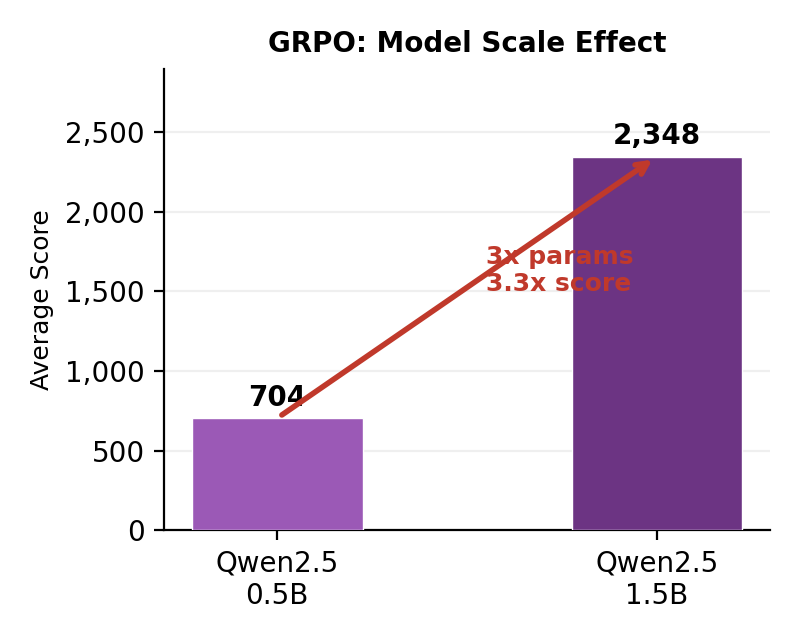
\includegraphics[width=\columnwidth]{fig_grpo_scaling.png}
    \caption{GRPO scaling: $3\times$ parameters $\to$ $3.3\times$ score.}
    \label{fig:grpo_scaling}
\end{figure}

\textbf{Chain-of-thought reasoning.} The 1.5B model produces interpretable move explanations. For example, given a board with 256 anchored in the bottom-right corner:

\begin{quote}
\small\texttt{<think> 256 anchored bottom-right -- good. Gradient: 128, 64, 32, 16 intact along right/bottom edges. RIGHT merges 4+4 in row~1 (+8). Avoids scattering corner tile. </think> <answer>RIGHT</answer>}
\end{quote}

\textbf{Spatial reasoning failure.} The 0.5B model reveals a fundamental limitation: it pattern-matches on token proximity rather than grid geometry. When tiles 4 appear at positions [0][1] and [1][0], the model incorrectly claims ``4 at [0][1] and [1][0] are adjacent -- LEFT merges them into 8.'' In reality, they are in different rows; LEFT moves each to column 0 independently with no merge. This spatial failure explains the 0.5B model's poor performance and suggests that larger models are needed for accurate mental simulation of board mechanics.

\subsection{Classical RL vs. RLVR Comparison}

Figure~\ref{fig:classical_vs_rlvr} directly compares all eight agents. Table~\ref{tab:head_to_head} provides a dimension-by-dimension comparison.

\begin{figure}[t]
    \centering
    
\includegraphics[width=\columnwidth]{fig_classical_vs_rlvr.png}
    \caption{Classical RL vs.\ RLVR: average score comparison across 1M steps, 5M steps, and GRPO training (300 prompts).}
    \label{fig:classical_vs_rlvr}
\end{figure}

\begin{table}[t]
\centering
\caption{Head-to-Head: Classical RL vs.\ LLM-RLVR}
\label{tab:head_to_head}
\resizebox{\columnwidth}{!}{
\begin{tabular}{@{}l l l@{}}
\toprule
\textbf{Dimension} & \textbf{Classical RL (best)} & \textbf{LLM-RLVR (GRPO)} \\
\midrule
Best Avg Score   & \textbf{7,744} (DQN, 5M)      & 2,348 (1.5B) \\
Best Max Tile    & \textbf{2048} (DQN, hunt)       & 256 (1.5B) \\
Parameters       & 120 -- 430K                     & 494M -- 1.8B \\
Inference        & \textbf{$<$4\,ms/move}          & 1,500\,ms/move \\
Training data    & 5M env steps ($\sim$2 hrs)       & 300 prompts ($\sim$12 hrs) \\
Training compute & 2 hrs (RTX 4060)                & 12 hrs (same GPU) \\
Interpretable    & No (black box)                  & \textbf{Yes (chain-of-thought)} \\
Observation      & \textbf{Tensor} (16ch)          & ASCII text \\
Action space     & Integer $\{0{-}3\}$             & Natural language token \\
\bottomrule
\end{tabular}
}
\end{table}

The $3.3\times$ score gap between the best classical agent (DQN, 7,744) and the best RLVR agent (GRPO 1.5B, 2,348) reflects fundamental differences in data efficiency and representation. DQN processes 5M transitions with replay, revisiting each state thousands of times; GRPO sees only $300{\times}4{=}1{,}200$ board states. DQN's 16-channel tensor encoding is information-dense; the LLM must tokenize and parse ASCII text, introducing representational overhead.

However, RLVR provides a unique advantage: \emph{interpretability}. Every GRPO move includes a chain-of-thought explanation that can be inspected, debugged, and corrected. Classical agents are complete black boxes. In applications where explainability is valued -- educational tools, human-AI collaboration, safety-critical systems -- the 400$\times$ latency penalty may be acceptable.

\subsection{Training Dynamics}

Figure~\ref{fig:dqn_curves} shows DQN's training curves over 5M steps, demonstrating steady improvement throughout. Figure~\ref{fig:sample_efficiency} compares the scaling behavior from 1M to 5M steps across all classical agents.

\begin{figure}[t]
    \centering
    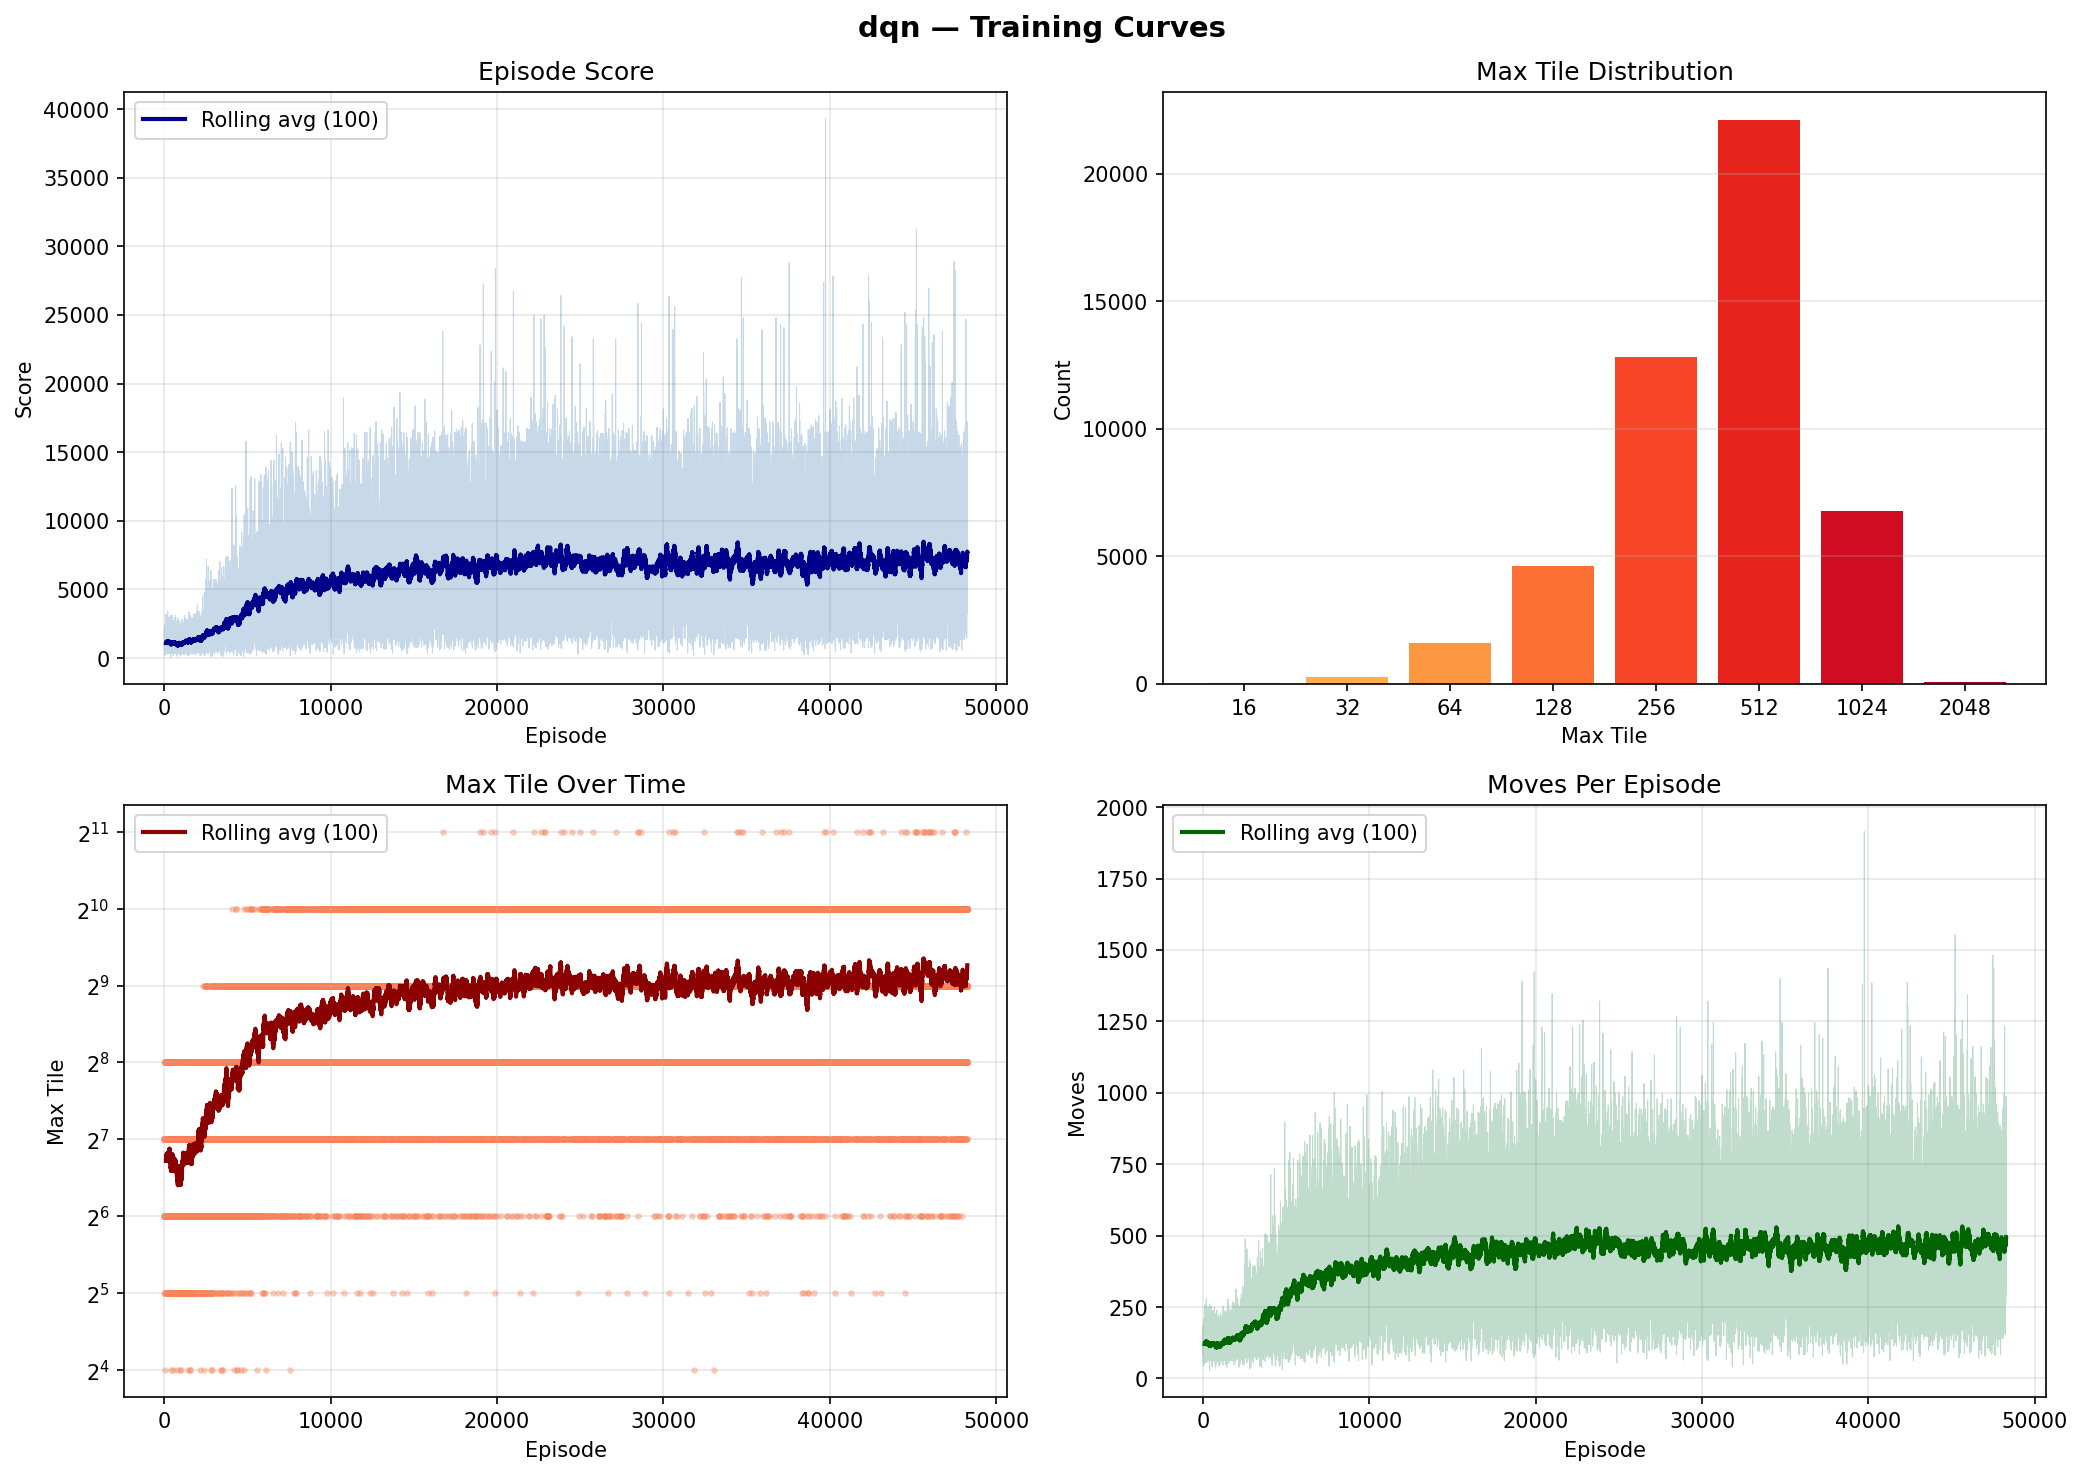
\includegraphics[width=\columnwidth]{fig_dqn_5m.png}
    \caption{DQN training curves over 5M steps. Score and max tile improve steadily, reaching 2048 tile and avg 7,744.}
    \label{fig:dqn_curves}
\end{figure}

\begin{figure}[t]
    \centering
    
\includegraphics[width=\columnwidth]{fig_sample_efficiency.png}
    \caption{Sample efficiency: 1M vs.\ 5M steps. DQN benefits most (+174\%); PPO and QR-DQN degrade ($-$12\%, $-$9\%).}
    \label{fig:sample_efficiency}
\end{figure}

%%====================================================================
\section{Conclusion}
\label{sec:conclusion}

We presented a systematic comparison of six classical RL agents and two GRPO-trained LLMs on the 2048 puzzle. Our controlled setup -- shared CNN backbone, identical environment, three evaluation tiers (1M, 5M, hunt mode) -- isolates algorithmic effects and yields four key findings:

\begin{enumerate}
    \item \textbf{Off-policy replay is decisive.} DQN's 100K replay buffer (S\&B~\S8.2) produces an $8\times$ advantage over on-policy PPO on identical architectures (7,744 vs.\ 962). Experience replay amplifies sparse rewards that on-policy methods see exactly once and discard.

    \item \textbf{Features beat deep networks at low data.} Semi-gradient SARSA with 120 hand-crafted parameters outperforms all deep on-policy agents (330K+ parameters), validating Sutton \& Barto's thesis~(\S9.5) that domain-specific features provide stronger inductive bias than CNNs learning from scratch.

    \item \textbf{More training actively hurts on-policy agents.} PPO and QR-DQN lose 9--12\% score from 1M$\to$5M steps, developing degenerate move loops. This is a cautionary finding for practitioners: longer training does not universally help.

    \item \textbf{LLM scale drives RLVR performance.} $3\times$ more parameters (0.5B $\to$ 1.5B) yields $3.3\times$ higher score. GRPO uniquely produces interpretable per-move rationale, but spatial reasoning remains a bottleneck at small model scales.
\end{enumerate}

Future work includes scaling GRPO to Qwen2.5-3B/7B on an A100 GPU, replay buffer ablation (10K--500K) to quantify the exact contribution of replay to DQN's dominance, multi-seed evaluation for statistical significance, and hybrid LLM-MCTS approaches combining interpretability with search efficiency.

%%====================================================================
\section*{Acknowledgment}

This project was completed as part of CS~5180 (Reinforcement Learning) taught by Professor Robert Platt at the Khoury College of Computer Sciences, Northeastern University. All experiments were conducted on a single NVIDIA RTX 4060 Laptop GPU (8\,GB VRAM).

%%====================================================================
\begin{thebibliography}{00}

\bibitem{guo2025deepseek}
D.~Guo \textit{et al.}, ``DeepSeek-R1: Incentivizing reasoning capability in LLMs via reinforcement learning,'' \textit{Nature}, vol.~645, pp.~633--638, 2025.

\bibitem{wen2025rlvr}
Y.~Wen \textit{et al.}, ``RLVR implicitly incentivizes correct reasoning,'' \textit{arXiv:2506.14245}, 2025.

\bibitem{saligram2025delayed}
P.~Saligram, T.~Bhathal, and R.~Manihani, ``2048: Reinforcement learning in a delayed reward environment,'' \textit{arXiv:2507.05465}, 2025.

\bibitem{hu2025lmgame}
L.~Hu \textit{et al.}, ``lmgame-Bench: How good are LLMs at playing games?'' \textit{arXiv:2505.15146}, 2025.

\bibitem{mnih2015human}
V.~Mnih \textit{et al.}, ``Human-level control through deep reinforcement learning,'' \textit{Nature}, vol.~518, no.~7540, pp.~529--533, 2015.

\bibitem{schulman2017proximal}
J.~Schulman, F.~Wolski, P.~Dhariwal, A.~Radford, and O.~Klimov, ``Proximal policy optimization algorithms,'' \textit{arXiv:1707.06347}, 2017.

\bibitem{mnih2016asynchronous}
V.~Mnih \textit{et al.}, ``Asynchronous methods for deep reinforcement learning,'' in \textit{Proc.\ ICML}, pp.~1928--1937, 2016.

\bibitem{dabney2018distributional}
W.~Dabney, M.~Rowland, M.~Bellemare, and R.~Munos, ``Distributional reinforcement learning with quantile regression,'' in \textit{Proc.\ AAAI}, 2018.

\bibitem{haarnoja2018soft}
T.~Haarnoja, A.~Zhou, P.~Abbeel, and S.~Levine, ``Soft actor-critic: Off-policy maximum entropy deep reinforcement learning with a stochastic actor,'' in \textit{Proc.\ ICML}, 2018.

\bibitem{christodoulou2019soft}
P.~Christodoulou, ``Soft actor-critic for discrete action settings,'' \textit{arXiv:1910.07207}, 2019.

\bibitem{dettmers2024qlora}
T.~Dettmers, A.~Pagnoni, A.~Holtzman, and L.~Zettlemoyer, ``QLoRA: Efficient finetuning of quantized language models,'' in \textit{Proc.\ NeurIPS}, 2024.

\bibitem{shao2024deepseekmath}
Z.~Shao \textit{et al.}, ``DeepSeekMath: Pushing the limits of mathematical reasoning in open language models,'' \textit{arXiv:2402.03300}, 2024.

\bibitem{szubert2014temporal}
M.~Szubert and W.~Ja\'{s}kowski, ``Temporal difference learning of n-tuple networks for the game 2048,'' in \textit{Proc.\ IEEE CIG}, 2014.

\bibitem{raffin2021stable}
A.~Raffin \textit{et al.}, ``Stable-Baselines3: Reliable reinforcement learning implementations,'' \textit{J.\ Mach.\ Learn.\ Res.}, vol.~22, no.~268, pp.~1--8, 2021.

\bibitem{qwen2024}
Qwen Team, ``Qwen2.5: A party of foundation models,'' \textit{arXiv:2412.15115}, 2024.

\bibitem{unsloth2024}
D.~Han and M.~Han, ``Unsloth,'' Available: \url{https://github.com/unslothai/unsloth}, 2024.

\bibitem{towers2024gymnasium}
M.~Towers \textit{et al.}, ``Gymnasium: A standard interface for reinforcement learning environments,'' \textit{arXiv:2407.17032}, 2024.

\bibitem{sutton2018rl}
R.~S.~Sutton and A.~G.~Barto, \textit{Reinforcement Learning: An Introduction}, 2nd~ed. Cambridge, MA: MIT Press, 2018.

\end{thebibliography}

\end{document}
